\section{Introduction}
\label{sec:intro}

Vision-language models (VLMs) have emerged as powerful planners for robotic manipulation, leveraging internet-scale semantic knowledge and visual perception to translate high-level instructions into executable action sequences~\cite{zitkovich2023rt, kim2025openvla, driess2023palm, jiang2023vima}. VLM-based systems have demonstrated strong performance on short-horizon manipulation tasks, including precise grasping, pose-aware placement, and decomposition of language instructions into subgoal sequences~\cite{brohan2023saycan, qisofar, huang2023voxposer, shridhar2023perceiver}.

However, this success does not readily extend to long-horizon tasks, which demand sustained spatial and causal awareness across multi-step action sequences that irreversibly alter the environment~\cite{shi2025hi, zhao2025cot, wu2023tidybot}. Current VLM-based planners lack the persistent state tracking required to bridge observations across steps, forcing them to reinfer world state from partial observations at each decision step~\cite{hanrobocerebra, huang2023inner, zhou2025code}. Without accumulated context, perceptual errors and action effects compound across steps, ultimately resulting in cascading failures, as illustrated in Fig.~\ref{fig:teaser}. In contrast, humans maintain a coherent mental model~\cite{lake2017building} that continuously integrates spatial relations and causal consequences as actions unfold, tracking not only where objects are but also how each action has cumulatively reshaped the world.



\begin{figure}[t]
        \centering  
        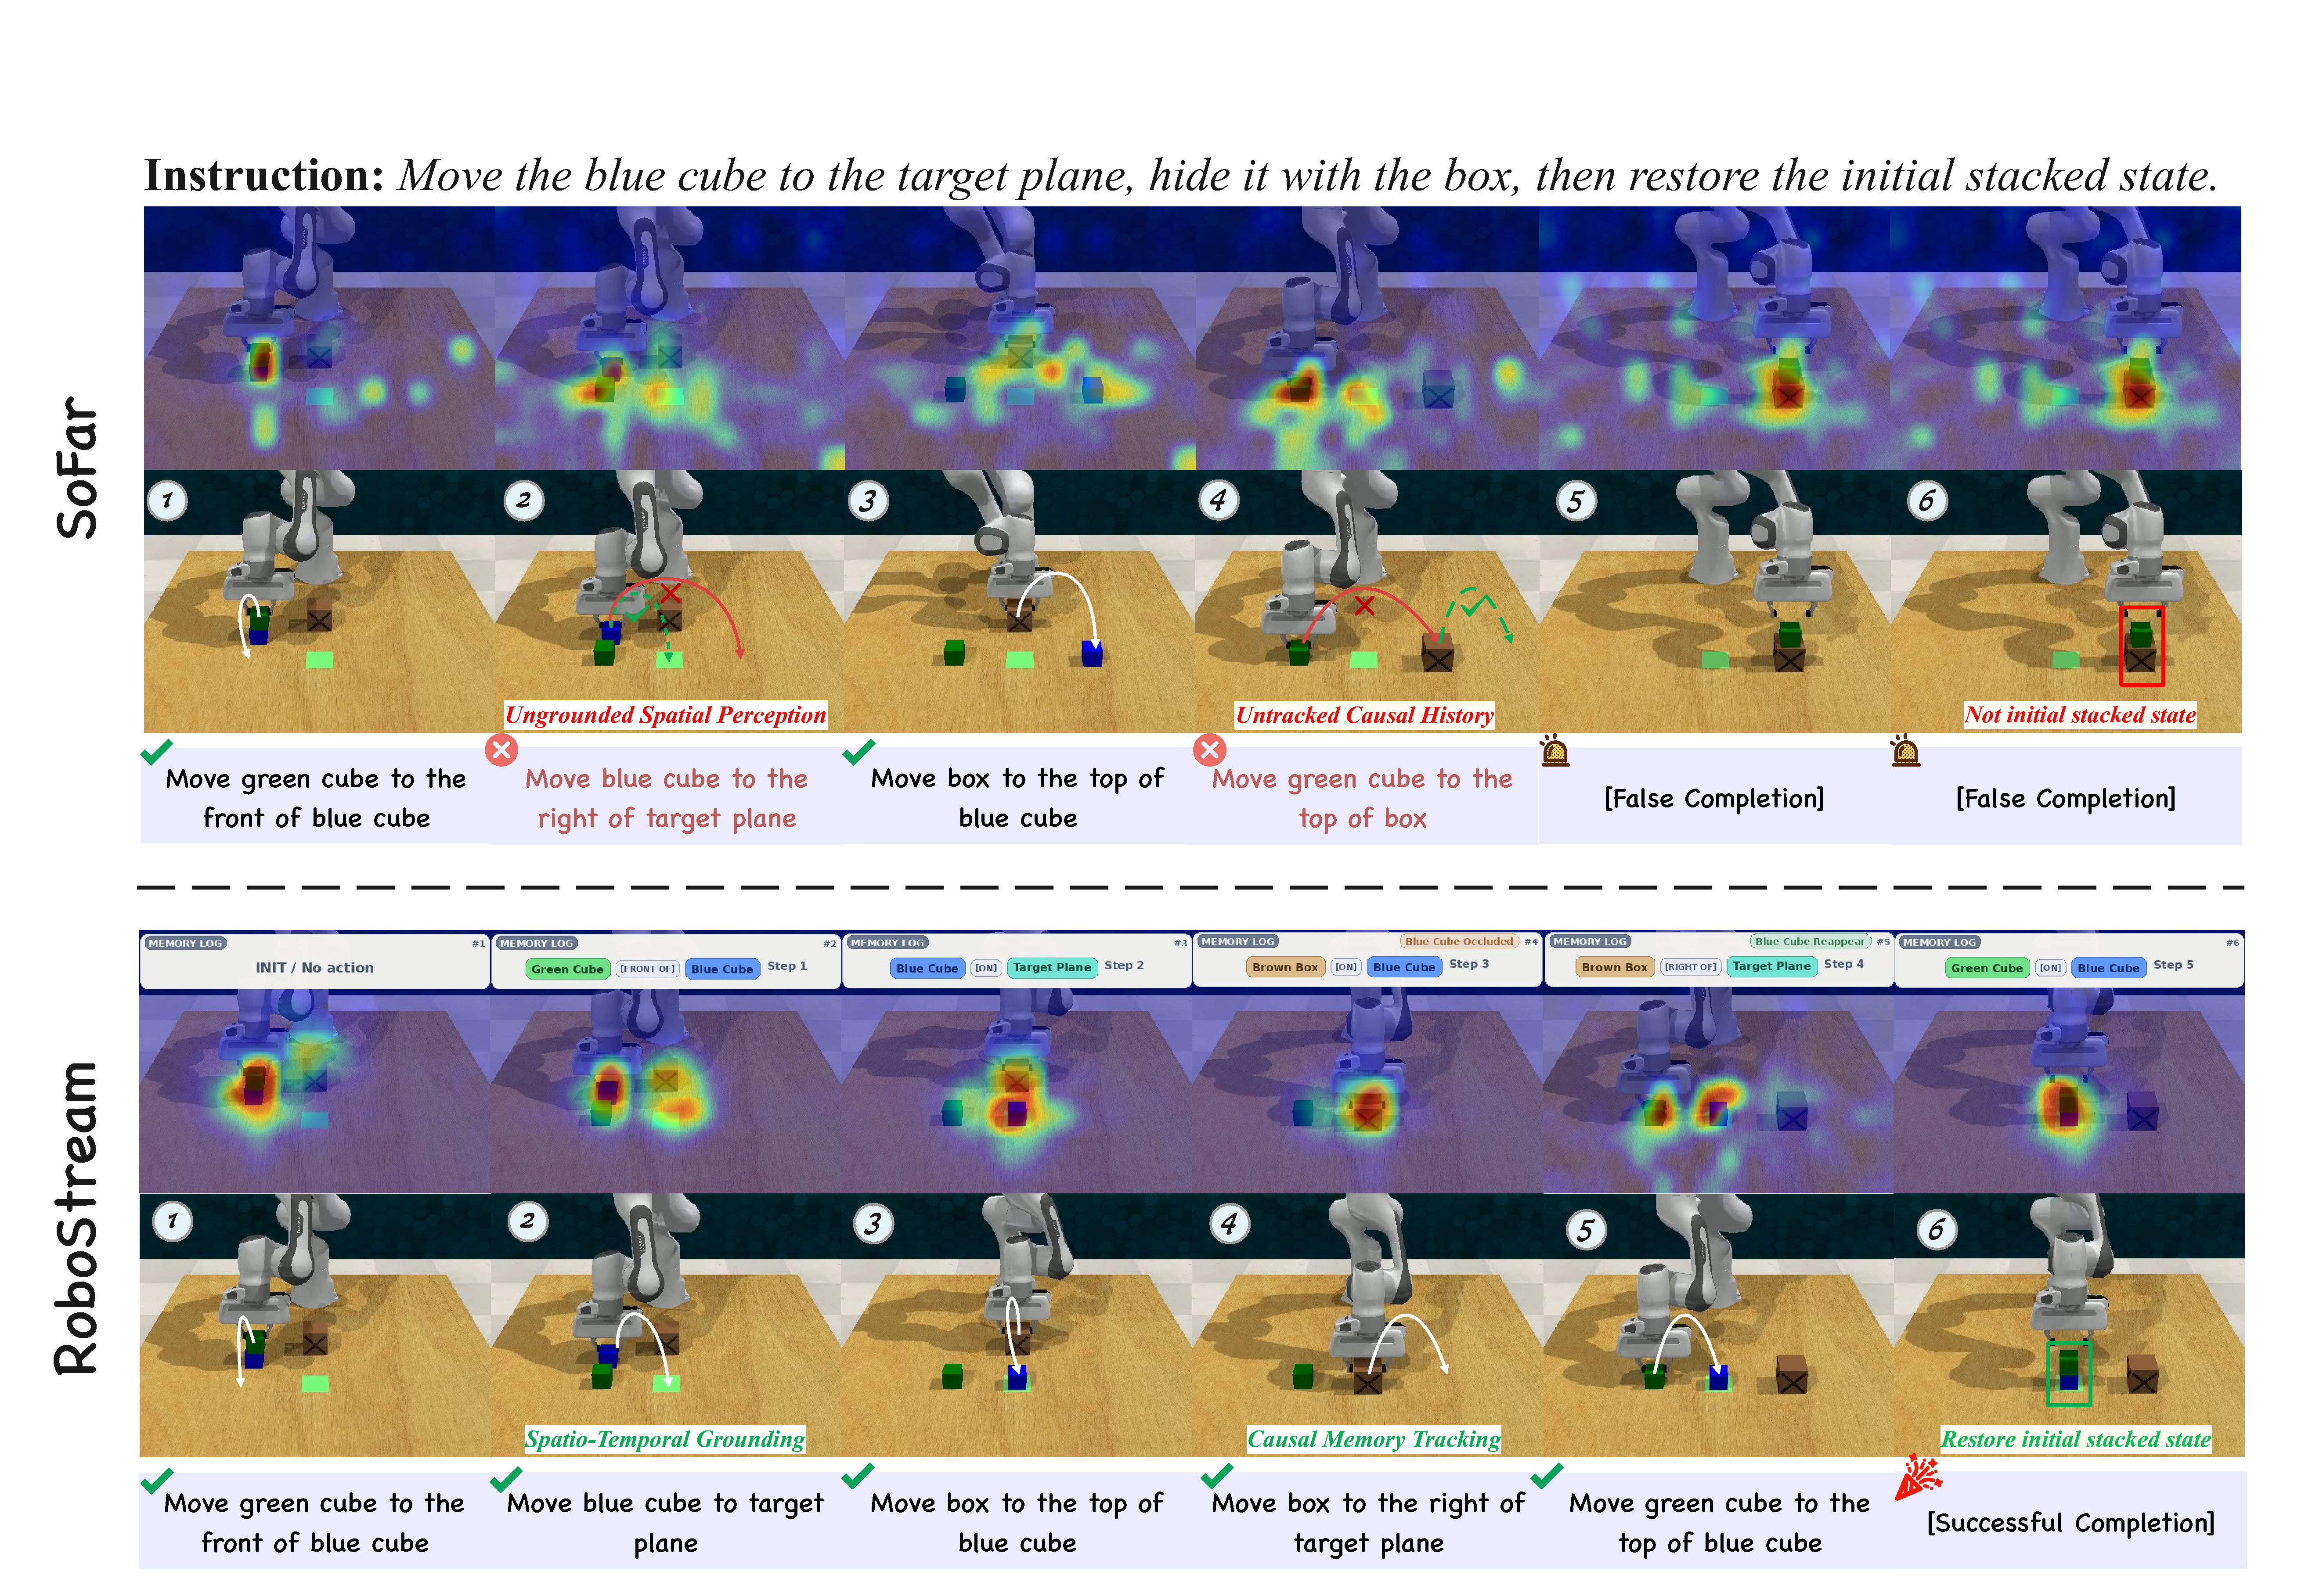
\includegraphics[width=1\textwidth]{Figures/RoboStream_Intro_Compare.pdf}
        \caption{\textbf{Qualitative comparison between SoFar~\cite{qisofar} and RoboStream.} This long-horizon task involves object occlusion and state restoration. \textbf{Top (SoFar):} Diffuse attention heatmaps and absent memory logs reveal two cascading failures: \textit{Ungrounded Spatial Perception} misplaces the blue cube at Step~2, while \textit{Untracked Causal History} leaves the planner unaware of the occluded cube at Step~4, resulting in an incorrect final state. \textbf{Bottom (RoboStream):} Concentrated attention heatmaps and persistent memory logs show that \textit{Spatio-Temporal Grounding} enables accurate object placement at Step~2, while \textit{Causal Memory Tracking} maintains awareness of the occluded cube at Step~4, enabling successful task completion.}
\label{fig:teaser}
\end{figure}


Replicating this human capacity for spatio-temporal reasoning requires persistent tracking of two interdependent quantities, namely the evolving geometric state of each object across steps and the causal record of how actions modify those states. Tracking alone is insufficient, as geometric states must be anchored in 3D space for reliable spatial reasoning while causal records must be structured to support inference over displaced or occluded objects. 
Current VLM-based planners fail at both, as illustrated in~Fig.~\ref{fig:teaser}, exposing two tightly coupled representation deficits.
\ding{172}~\textit{Ungrounded Spatial Perception}: spatial relations in manipulation are latent state components continually rewritten by contact and motion, yet current systems infer them implicitly via image-centric perception without geometric anchoring or cross-step identity binding~\cite{chen2024spatialvlm, huang2024copa, yuan2025robopoint}. This forces geometry reconstruction from raw pixels at every step, where small inaccuracies accumulate into spatial hallucinations and precondition violations.
\ding{173}~\textit{Untracked Causal History}: although actions irreversibly alter the environment, existing methods retain no record linking actions to induced state transitions. Without causal tracking, planners remain unaware of displaced objects and lose track of occluded ones entirely, leading to precondition violations when subsequent actions depend on altered states~\cite{wen2025dexvla, zhen20243d}.


To address these two deficits, we propose \textbf{RoboStream}, a training-free framework that weaves spatio-temporal reasoning and persistent memory directly into the VLM planning loop through \textit{Spatio-Temporal Grounding} and \textit{Causal Memory Tracking}. For grounding, Spatio-Temporal Fusion Tokens (STF-Tokens) distill visual appearance and 3D geometry (centroid and Gaussian shape) of each object into identity-persistent primitives, shifting VLM reasoning from pixel-level reconstruction to structured object-instance references that suppress cascading spatial errors. For tracking, a Causal Spatio-Temporal Graph (CSTG) records action-triggered state transitions alongside persistent object identities, preserving object permanence under occlusion without direct visual evidence.
We evaluate RoboStream on five benchmarks spanning simulated and real-world settings: SIMPLER~\cite{li2025evaluating}, long-horizon RLBench tasks~\cite{james2020rlbench}, 6-DoF SpatialBench~\cite{qisofar}, Open6DOR V2~\cite{ding2024open6dor}, and long-horizon real-world Franka experiments including block building, disassembly, and hide-and-restore under occlusion.
Across all settings, RoboStream outperforms existing VLM-based planners, demonstrating that spatio-temporal reasoning and persistent memory are essential for robust long-horizon manipulation.
Our contributions are as follows:

1) We introduce \textbf{RoboStream}, a training-free framework weaving spatio-te\-m\-p\-o\-r\-a\-l reasoning with persistent memory to overcome spatial hallucination and causal blindness in VLM-based planners. By anchoring geometric evidence across steps and tracking causal state transitions, RoboStream builds persistent world representations enabling robust long-horizon reasoning without retraining.


2) We design two synergistic mechanisms for Spatio-Temporal Grounding and Causal Memory Tracking. \textit{Spatio-Temporal Fusion Tokens (STF-Tokens)} bind visual evidence to 3D geometry, converting pixel-level inference into deterministic spatial references. A \textit{Causal Spatio-Temporal Graph (CSTG)} maintains object identities and records action-triggered state transitions, enabling causal inference of occluded states and preventing error accumulation over long horizons.

3) RoboStream achieves state-of-the-art results across five benchmarks spanning long-horizon manipulation (RLBench, real-world Franka), zero-shot generalization (SIMPLER), and spatial reasoning (6-DoF SpatialBench, Open6DOR V2), validating that weaving spatio-temporal reasoning with persistent memory is essential for robust manipulation across diverse settings.



